\clearemptydoublepage
\chapter{Background}

\chaptermark{Background}
%What is model driven engineering
%Metamodeling: definition and tools
%Main concepts: metamodel, constraint, transformation,
%Automation in MDE
%Evolution in MDE
In this chapter, we introduce the field of Model-Driven engineering. In section ?, we present the activity of metamodeling and the involved artifacts. Section ? discusses the automation task related to the artifacts presented in section ?. We finish this chapter with a presentation of the evolution concept in the context of model driven engineering.
%define the terminology of the main concepts that we use. 
% We define the specific scope of problems addressed in this thesis
% and discuss the spectrum of problems that arise in this field. 
%TODO Terminology: Model-Driven engineering, co-evolution
% Metamodel, co-evolution, code, maintenance, refactoring

\section{Model-Driven Engineering}
To develop a software, a list of specifications is given to the developers, to code the final product. This approach can work in the case of small projects. When the complexity of the software increases, more efficient approaches must be adopted. Model driven engineering has proven  its efficiency comparing to other engineering disciplines \cite{1231146}.

%\boitemagique{Model-Driven Enginereering}{
\textit{Model-Driven Engineering(MDE)} is the systematic use of models as primary artifacts during a software engineering process. MDE includes various model-driven approaches to software development, including model-driven architecture, domain-specific modeling and model-integrated computing~\cite{10.1145/1985793.1985882}. The first appearance of MDE like approaches started in the 80's \cite{10.1007/s10270-005-0079-0}. MDE still adopted  and a lot of work is being done in academia and industry, refs.

%}
%TODO detaills the benefits of MDE

%Details about MDE approach 
The goal of MDE is to improve productivity, quality, and maintainability by leveraging high level abstractions throughout the development process. The metamodeling phase implied the experts of the domain who focus on the major key aspects of the problem rather than being concerned about the underlying programming language and the implementation.
%about major key aspects of the problem statement rather than focusing on programming.
%Metamodeling and modeling langugaes

% MEtamodel def :
The metamodel represent the main artifact in MDE. There are many definitions of the concept "metamodel" that can be found in literature:

\textit{A metamodel} describes concepts that can be used for modeling the model (i.e. in the instances of the metamodel).

\textit {Metamodels} are models that make statements about modeling. More precisely, a metamodel describes the possible structure of models in an abstract way, it defines the constructs of a modeling language and their relationships, as well as constraints and modeling rules – but not the concrete syntax of the language.

\textit{A metamodel} defines the abstract syntax and the static semantics of a modeling language ,Vice versa, each formal language, such as Java or UML, possesses a metamodel.

Seidewitz \cite{seidewitz2003models} gives another commonly used definition of \textit{metamodels} in MDE. A metamodel is a specification model for a class of systems under study where each system under study in the class is itself a valid model expressed in a certain modeling language.

\section{Metamodeling}

%%
\textit{Metamodeling} is the process of metamodel creation. Metamodeling is done thanks to metamodeling languages ( that is in turn described by a meta metamodel).

Metamodeling must gathers the whole  knowledge that is required to define, precise, and deal with MDE challenges in its different tasks:

%DSL/ sftware language 
%Construction of domain-specific modeling languages (DSLs): 
%The metamodeling activity includes other tasks:
\begin{itemize}
\item The construction of metamodel describes the abstract syntax of target (software languages, solution system).
\item Model validation: models are validated against the constraints defined in the metamodel. 
\item Model-to-model transformations: such transformations are defined as mapping rules between two metamodels.
\item Code generation: the generation templates refer to the metamodel of the "system". 
\item Tool integration: based on the metamodel, modeling tools can be adapted to the respective domain. 
\end{itemize}


In the context Domain-Specific Language, DSMLs can be tailored via metamodeling to precisely match the domain's semantics and syntax. The concrete syntax that is, the concrete form of the textual or graphical constructs with which the modeling is done must represent the metamodel in an unambiguous way. Having graphic elements that linked directly to a familiar domain makes it easier to learn and allows domain  experts to contribute, such as system engineers and experienced software architects, ensure that software systems meet user needs \cite{volter2013model}. The metamodel is the basis for the automated, tool-supported processing of Metamodeling models. On the other hand, a suitable concrete syntax is the interface to the modeler and its quality decides what degree of readability the models have \cite{}.


%Metamodeling tools/languages/techniques examples :

// Add figure?

Metamodeling languages are classfied into two categories languistic and ontological\cite{gavsevic2007metamodeling}. Linguistic metamodeling represents  way for defining modeling languages and their primitives (e.g., Object, Class, MetaClass) on the layer of a metamodel. Ontological metamodeling aims to represent domain knowledge accurately, it is s concerned with semantics and meaning, ex: OWL \cite{}. Linguistic metamodeling aims to define a language for creating models. it is concerned with syntax and structure.
We can use a different classfication by purpose: General Purpose Modeling Langugaes and Domain-Specific Modeling Languages \cite{de2012domain}. General purpose modeling languages as for example : UML and its variants, generic metamodeling frameworks, such as MOF \cite{}, and Ecore \cite{}. As examples of DSLs, we cite sysML and EXPRESS DSL.

In MDE, there are language workbenches that are used for language creation, such as Xtext, MetaEdit+.
% Add figure for above languages/techniques/frameworks

%\textbf{Generated artifacts, artifacts linked to the metamodel}


Metamodel is the backbone in model driven engineering. In the language modeling ecosystem, other artifacts are created by the mean of the metamodel. By definition, the model is an instance of a metamodel, which mean that the metamodel defines the concepts with which a model can be created. Constraints are written in Object Constraint Language. The created models can be validated through a set of constraints to check the models' correctness. They precise specifications on the model that cannot be  expressed by diagrammatic notation. In order to safe effort and avoid errors, models transformation is one of the common automated tasks in Model-driven engineering. Model transformation are expressed in  Transformation Languages for example, ATL). A transformation consists of a set of rules that map the source metamodel elements to the metamodel target’s elements. 

// Add example of Metamodel+ model+constraint+transformation ?

%ex constraint : the age of a person is not negative, a person is younger than its parents
%Automation in the ecosystem
%code gen 
%tests
\section{Automation in the MDE ecosystem}

Brief description about approaches that allow automated tasks in MDE.

\textbf{Code Generation}

One of the most important advantages of MDE, is the automation in many of its activities. The code generation activity is recurrent, and its automation enhances the productivity and the cost.
For example, Eclipse Modeling Framework built-in code generator allows to generated a java API from an Ecore metamodel. The generated code API structure and technical choices are done to fit Java programming language and model driven engineering abstraction standards/principles (ex: each metaclass is used to generate an interface and concrete implementation class that extends the generated interface, pattern observer), to have an efficient as possible.
\textit{@generated} annotation is used to mark generated interfaces, classes, methods, and fields.

In Eclipse Modeling Framework, two model resources (files) are manipulated: the .ecore file that contains  xmli serialization of the E
core model and the .genmodel for the serialized generator model.

\section{Evolution in the MDE context}

During the software development process, software artifacts are meant to be changed, due to many reasons: client requirements and domain specification, software maintenance or bug correction. Like any other software system, modeling languages are the subject of an inevitable evolution, during their process of building, multiple versions are developed, tested, and adapted until a stable version is reached. 

Different types of evolution are categorized depending on the impact and purpose of the applied modifications \cite{lientz1980software,Swanson1976}:
\begin{itemize}
	
	\item  Corrective: aims to correct discovered problems and inconsistencies such as processing failures, performance failures, or implementation failures by applying  a set of reactive modifications of a software product.  
	
	\item  Adaptive: in case of changing environment, such as changes in data environment or processing environment, this evolution aims to keep a software product usable.
	
	\item Perfective: this evolution aims to improve functionalities, enhance the performance, reliability, or to increase the maintainability of a software.  
	
\end{itemize}

The term \textit{Evolution} can be refined as the literature presents various related terms like : Maintenance, Refactoring, and \textbf{Co-evolution}, which are different types of modifications that could be applied on a software.

//Why we need to perform evolution ?
Answer to requirment changing, and technological progress : examples?

\textit{Evolution}: when users and developers get by learning  new requirements  
that lead to adapt the software to new changes \cite{}. 

\textit{Maintenance}:It is modifying a software product after delivery to correct faults, to improve performance, or to adapt the product to a changing environment  \cite{}.

\textit{Refactoring}: It is an oriented object term, that means modifications of software to make it easier to understand and to change or to make it less susceptible to errors when future changes are introduced  \cite{}. 

\textit{co-evolution}: It consists of the process of adapting and correcting a set of artifacts $A_1$, $A_2$, ...$A_N$ in response to the evolution of an artifact B on which $A_1$, $A_2$, ...$A_N$  strongly depend  \cite{}, for example the co-evolution of models with the evolving metamodel.


\begin{figure}[htbp]
	\begin{center}
		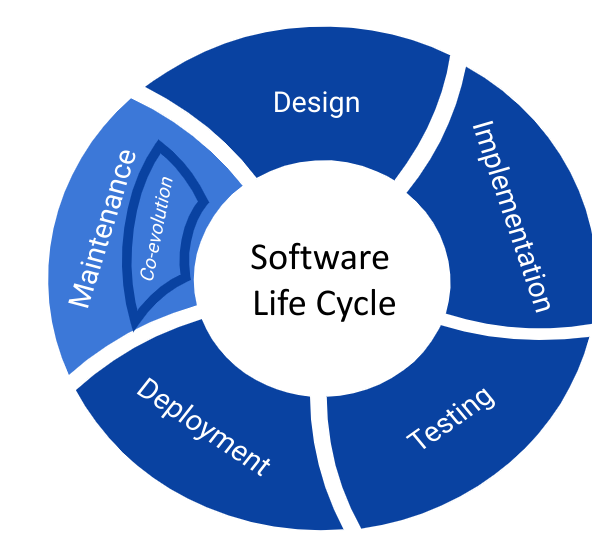
\includegraphics[width=0.6\linewidth]{./pics/soaPics/solicy.png}
	\end{center}
	\caption{Software Life Cycle}
%	{\footnotesize Titre plus long avec des explications.}
	\label{fig:softwarelifecyle}
\end{figure}

\begin{figure}[htbp]
	\begin{center}
		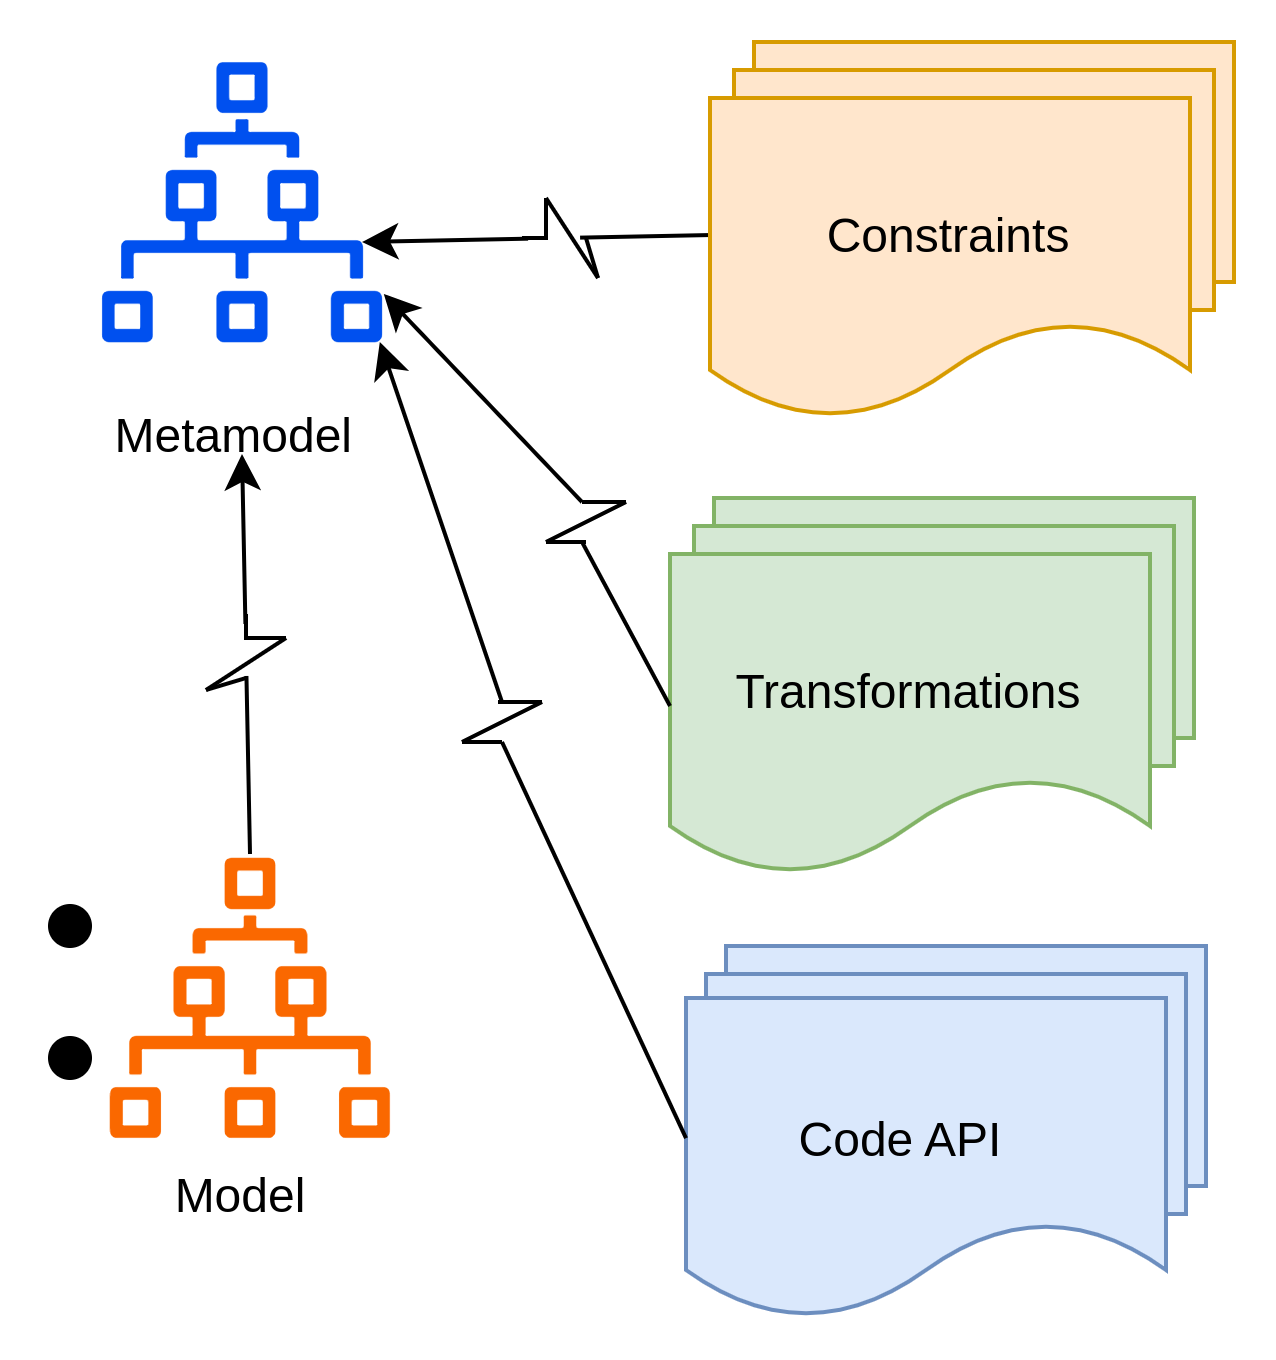
\includegraphics[width=0.6\linewidth]{./pics/soaPics/mdeecosystem.png}
	\end{center}
	\caption{MDE Ecosystem}
%	{\footnotesize Titre plus long avec des explications.}
	\label{fig:mde_ecosystem}
\end{figure}


%definition
\chapter{State Of The Art}

\chaptermark{State Of The Art}
%offline and online process
we present an overview of what has been done in the field of code co-evolution in the context of model-driven engineering. We split this overview into ? parts. In section ?, we present the metamodel change detection approaches. Section ? presents the co-evolution of model, transformations, constraints with evolving metamodel. In section ?, we discuss code co-evolution and relevant literature about API-client evolution, language evolution, and evolution in low-code platforms. We finish this chapter with a discussion with focus on limitations and research gap.
 \section{Metamodel change detection}
 One of the intrinsic properties of software artifacts is its continuous evolution~\cite{mens2008introduction}. Like any software artifact, metamodels are meant to evolve to meet the represented domain. %one key sentence of the context
 In this thesis, our context is triggered by the metamodel evolution, that's why we find essential to understand this evolution in detail.
 %metamodel diffing
 A lot of work has been done on metamodel diffing.
 Detection approaches can be classfied into two main categories; online detection approaches, and offline detection approaches. Thid classification can be refined using some factors : automation degree, types of detected changes, considered issues (overlap, indefinit length, hidden changes, order of changes, undo operations)\cite{hebig2016approaches}.
 
 
 
  In another hand, many of them classified the detected changes based on their impact on the treated artifact (for ex, on models, constraint, transformation). Here we put the largest set of changes types, later, we will specify treated types with their possible impact on the code.
 
 
 Two types of evolution changes are considered when evolving a metamodel: \emph{atomic} and \emph{complex} changes~\cite{hebig2016approaches,Herrmannsdoerfer2011}. 
 Atomic changes are additions, removals, and updates of a metamodel element. Complex changes consist of a sequence of atomic changes combined together~\cite{vermolen_reconstructing_2012},~\cite{khelladi2015detecting}. For example, move property is a complex change where a property is moved from a source class to a target class. This is composed of two atomic changes: delete property and add property~\cite{Herrmannsdoerfer2011}. 
 Many approaches in the literature~\cite{Alter2015, williams2012searching,cicchetti_managing_2009,langer_posteriori_2013,vermolen_reconstructing_2012,Khelladi2016,bettini2022executable} exist to detect metamodel changes between two versions.
  
 \vspace{1em}
 	\begin{tabular}{ |c|c| } 
 		\hline
 		Type  & Change name \\
 		\hline
 		\multirow{4}{4em}{ Atomic changes} & Delete class  \\ 
 		& Delete property \\ 
 		& Add class \\ 
 		& Add property \\ 
 		& Rename class \\ 
 		& Rename property \\ 
 		& Generalize property \\ 
 		\hline
 		\hline
 		\multirow{5}{4em}{Complex changes} & Move property \\ 
 		& Push property  \\ 
 		& Pull property\\ 
 		& Inline class\\
 		& Change property type\\
 		\hline
 		
 	\end{tabular}
 	  
 	\vspace{1em}
 	
 	Categorization of changes : 
 	non breaking
 	breaking resolvable
 	breaking and unresolvable
 	
 \section{Co-evolution of models, constraints, and transformation}
 In MDE ecosystem, the metamodel is the starting point to have other artifacts that we defined in section ?. in this section, we will present an overview of the existing works about these artifacts co-evolution. Note that if the solution est applied during the evolution of the metamodel, we call it an online solution, otherwise it is offline.
 The comparison, advantages, and drawbacks of the presented approaches is out of the scope of this dissertation.
 
\subsection{Metamodel and model co-evolution}
Due to metamodel evolution, the model becomes "no conform".
%Once the metamodel changes are detected, using one of the previously presented approaches in Section ?, 
 %a set of resolutions are applied to co-evolve the model to gain again the conformity to the metamodel.
 %change order, resolution order
 Co-evolution  approaches use automatic or manual diffing metamodel approaches in their solutions. Model co-evolution approaches that we found can be categorized into four categories. The first category is Resolution Strategy Languages that specifies in a transformation language how to update the model given the list of metamodel changes. The category Resolution Strategy Generation groups approaches that generate full or partial resolution for each metamodel change.
 The co-evolution between metamodel and models can be processed manually but it requires a huge expertise. We find three categories of metamodel and model co-evolution approaches. Approaches based on resolution strategy languages that propose transformation languages created given the metamodel changes. The second category groups Resolution strategy generation approaches that allow to generate full or partial resolutions for each metamodel change. Some of these approaches  requires the user intervention to make decision on the selected operation to adapt the model. The category of  Resolution strategy leaning that adopt machine learning algorithm to select the resolution strategy for metamodel changes.
. Other approaches consider the model co-evolution problem as an optimization one that does not need the list of changes of the metamodel \cite{}.
%Demuth el al. [6] who used it for models co-evolution.
% There are also approaches for semi-automatic co-evolution of models that rzquires the user intervention to make decision on the selected operation to adapt the model.

%\cite{kessentini2018integrating,kessentini2019automated,cicchetti2008automating,herrmannsdoerfer2009cope,garces2009managing,wachsmuth2007metamodel},
\subsection{Metamodel and constraints co-evolution}
Another artifact that depends on the metamodel and needs to be adapted to the evolution of its metamodel is Constraints.
 Constraints co-evolutions that we can find in literature may be  online or offline. Every approach has its own co-evolution mechanism that treats specific types of metamodel changes and has its automation degree. Demuth et al propsed a template-based, hat cannot cover all changes types, of the predefined structure of the updated constraint.  Markovich et al proposed refactoring rules that depends on the impact of UML class diageam evolution on the constraints. Hassam et allpropose METAEVOL, based on a tranformation language.Kusek et al propose a solution for the co-evolution of the constrain body and do not incluse its context that may need co-evolution also.
 Cabot et al ocl contraints co-evolution due to metamodel deletion change. Khelladi et al propsed an approach that record the metamodel atomic and complex changes in a chronolical otder then apply one or many resolutions to co-evoolve the constraints. Batot et al takles the constraint co-evolution problem as an mulri-ovjective optimisation problem and apply heuristic-based recommendation approach that does not require /use a predefined set of transformation rules / resolution to coec-lve the constraints. Demuth, markovitch, cabot their approaches ar fully automatic while Hassam kusel and Khelladi  and Batot propose semi-automatic approches since the user must select from the recommendec output constraints. 
 
 
\subsection{Metamodel and transformations co-evolution}

Almost all the existing transformation approaches that we find in literratue starts by analysing the impact of the metamodel on the model transformations.
Mendez et al. [30] and Ruscio et al. [8,Garces et al. [10],Kusel, et al. [29] and khelladi proposed to co-evolve impacted transformation with a set of resolutions, khelladi covers the larget set of possible resolutions where Ruscio et al. [8, estimate the cost of the co-evoltuion to decide about the co-evolution,they further explored the variability of the co-evolution due to the possible alternative resolution . Garcia et al. [11] proposed a ATL tranformation-base approach which means that their resolutions are ATL transformations. All the approaches propose unique resolution to co-evolve the transformation
Ruscio et al. [8 allow developers to manually replace or refine a resolution. Khelladi et al allows to compose existing resolutions into a new one. Kessentini et all used a different approach that do not use the changes of the metamodel as input and do not process by an impact analysis, but it uses a search-based approach that relied on multi objective heuristic algorithm NSGA-II.
 \section{Metamodel and code co-evolution}
 
  \section{API and Client co-evolution}
 %TODO What has been done so far: 
%TODO Change detection
%TODO Metamodel-Transformation co-evolution
%TODO Metamodel-Constraint co-evolution
%TODO Metamodel-Model co-evolution
%TODO Metamodel-code co-evolution
%Discussion about automation degree of the approaches, best in cases and other cases not really

%TODO API-Client co-evolution

%TODO Language Evolution (e.g., Java V1 to V2)
%TODO Evolution in low-code platforms
%TODO Classification of related work 

%TODO Focus on limitations/research gap.
